% main.tex
\documentclass[12pt]{article}



% Import formatting & packages
% preamble.tex
\usepackage[a4paper, margin=2.5cm]{geometry}  % Page size & margins
\usepackage{graphicx}   % Figures
\usepackage{subcaption} % Defines the subfigure environment
\usepackage{booktabs}   % Professional tables
\usepackage{amsmath}    % Math symbols & equations
\usepackage{amssymb}    % More math symbols
\usepackage{hyperref}   % Hyperlinks
\usepackage{cleveref}   % Smart references
\usepackage{enumitem}   % Customizable lists
\usepackage{float}      % Better table/figure placement
\usepackage[utf8]{inputenc}  % Ensure Overleaf uses UTF-8 encoding
\usepackage{csquotes}   % Improved quotation formatting
\usepackage{tabularx}
\usepackage{tabularray}
\usepackage{tikz}
\usetikzlibrary{shapes.geometric, arrows}
\usepackage{pgfplotstable,siunitx,xfp}
\pgfplotsset{compat=1.18}
\usepackage{siunitx}   % \num, rounding/formatting
\usepackage{xfp}       % or expl3; xfp gives \fpeval
\usepackage{titling} 
\usepackage{verbatim} % for \verbatiminput
\usepackage{catchfile}
\usepackage{multirow}
\usepackage{booktabs}
\usepackage{array}
\usepackage{setspace}


% Bibliography
\usepackage[backend=biber, style=authoryear, sorting=nyt]{biblatex}  
\addbibresource{references.bib}  % Link to your Zotero export

% Section number depth
\setcounter{secnumdepth}{3}

% Table & figure captions
\usepackage[labelfont=bf]{caption}  

 % Word count command
\newcommand{\wordcount}{%
  % Run texcount on the main document (jobname.tex)
  %  - stdout -> \jobname.wc
  %  - stderr (warnings) -> nul (ignored)
  \immediate\write18{texcount -inc -sum -0 -template={SUM} \jobname.tex > \jobname.wc 2> nul}%
  % Read the result from the temporary file:
  \CatchFileDef{\wcresult}{\jobname.wc}{}%
  \mbox{\wcresult\unskip}%
}










\begin{document}

%TC:ignore
\begin{titlepage}
  \begin{center}
    \vspace*{1cm}

    % University + document type
    {\Large UNIVERSITEIT UTRECHT\par}
    \vspace{0.5cm}
    {\large MASTER THESIS\par}

    \vspace{2cm}

    % Title
    {\Huge \textbf{Addressing the Cold Start Problem in AI-Assisted Systematic Reviews}\par}
    \vspace{0.5cm}
    {\LARGE
      Getting started when evidence is scarce \par
    }

    \vspace{2.5cm}

    % Author(s)
    {\large \textbf{Author:}\par}
    \vspace{0.2cm}
    {\large Timo van Ommeren\par}

    \vspace{1cm}

    % Supervisor(s)
    {\large \textbf{Supervisors:}\par}
    \vspace{0.2cm}
    {\large Prof. dr. A.G.J. (Rens) van de Schoot, Lauke Stoel\par}

    \vspace{1.5cm}

    % Programme / degree line (adapt as you like)
    {\large
      MSc Methodology and Statistics for the Behavioural,\\
      Biomedical and Social Sciences\par}

    \vspace{0.5cm}

    % Host department / organisation (mirroring "Ministry of Health..." line)
    {\large Methodology Department, Utrecht University\par}

    \vfill

    % Logo
    
\includegraphics[width=0.2\textwidth]{images/Utrecht_University.png}

    \vspace{0.8cm}

    % Date and word count
    {\large \today\par} {\large Word count: \wordcount}

  \end{center}
\end{titlepage}
%TC:endignore


\section{Introduction}

\subsection{The framework: AI-assisted systematic reviews}

Researchers and practitioners are continually challenged to base their decisions on the latest scientific evidence \parencite{sackett1996evidence, subbiah2023next, sheridan2016achievements, chalmers2002brief}. To that end, systematic reviews and meta-analyses were developed as rigorous methods of summarizing scientific literature \parencite{grant2009typology, brignardello2025systematic, borenstein2021introduction, kicinski2015publication}. However, systematically reviewing large bodies of literature can be time-consuming. In particular, screening titles and abstracts to identify relevant papers is often a major bottleneck limiting the practical applicability of systematic reviews \parencite{nussbaumer2021resource, bastian2010seventy, borah2017analysis}.

Fortunately, recent advances in machine learning have produced tools that assist researchers in screening papers by prioritizing the most relevant papers for screening first \parencite{van2021open, ouzzani2016rayyan, ge2024leveraging, dos2023usefulness}. One such tool is \textit{ASReview}, an open-source software package for AI-assisted systematic reviews \parencite{van2021open, asreviewvs2jonathan}. ASReview uses active learning models to iteratively learn from the user's screening decisions and adaptively prioritize the most relevant papers for screening. AI-assisted screening can significantly reduce the time and effort needed to conduct systematic reviews and may even help identify more relevant papers compared to traditional screening methods \parencite{teijema2025large, byrne2024impact, ferdinands2023performance, van2025hunt}. 

\subsection{The problem: the cold start problem}

A key challenge limiting the application of AI-assisted systematic reviews is the "cold start" problem \parencite{van2021open, lika2014facing}. In the context of AI-assisted systematic reviews, the cold start problem refers to the inability of the active learning model to prioritize relevant papers for screening when it has yet to be trained on any examples of relevant papers \parencite{bobadilla2013recommender, zhang2023cold}. Notably, however, the cold start problem is usually not an issue because researchers can initialize, or 'warm up', the active learning model using \textit{true examples} of relevant papers prior to screening \parencite{panda2022approaches}. However, in some cases little to no prior research may be available \parencite{funtowicz1994uncertainty, evans2022sage}. In this case, the researcher may have to start screening papers at random until a relevant paper has been found which the model can be trained on. The cold start problem is particularly problematic in crisis situations such as COVID-19, where there may not be relevant prior literature and timely evidence synthesis is crucial \parencite{tricco2020rapid, kurzer2023follow}.

% A key challenge to using active learning for systematic reviews is that these models face a "cold start". In general, the cold start problem  refers to the inability of some recommender systems to provide accurate recommendations when dealing with new users or items \parencite{}.

% the cold start problem arises when the active learning model has no prior examples of relevant papers to be trained on prior to screening \parencite{van2021open}. As a result, the user may have to start screening papers at random without the active learning model being able to prioritize relevant papers for screening, until a relevant paper has been found and the model can be trained on this example. This may lead to suboptimal starting performance and increased screening time, especially when the percentage of relevant papers returned by a systematic search is low. 

\subsection{The proposed solution: eligibility criteria and large language models}

% It may be possible to overcome Large language models (LLMs) can address the cold start problem in AI-assisted systematic reviews, even when there are no prior examples of relevant papers. Specifically, LLMs can generate plausibly relevant titles and abstracts for a systematic review based on that review's eligibility criteria criteria. These examples can then be used to train an active learning model before screening begins, thus avoiding a cold start. Indeed, LLMs have already been shown to be effective in addressing the cold start problem in recommender systems and active learning . Notably, however, while there are many studies on the application of LLMs to various stages of the systematic review process \parencite{lieberum2025large, cao2025automation, sollini2025human, kim2025evaluating, bron2024combining, delgado2025transforming}, to the best of our knowledge, there are no studies that have investigated the use of LLMs to initialize active learning models and overcome the cold start problem in AI-assisted systematic reviews. Consequently, it remains unclear how starting performance is affected by the use of LLM-generated examples compared to a cold start, the use of actual examples of relevant papers, and the direct use of the eligibility criteria criteria as an example of a relevant paper. This study aims to investigate these questions through a simulation study using ASReview.

A possible solution to the cold start problem is to use the systematic review's eligibility criteria criteria to initialize the active learning model. The eligibility criteria criteria of a systematic review are typically well-defined and provide a clear description of what constitutes a relevant paper for that review \parencite{cochraneChapterDefining}. By using the eligibility criteria criteria as an example of a relevant paper, the active learning model can be trained on this example before screening begins, thus potentially avoiding a cold start. Moreover, it may be possible to further improve starting performance by using large language models (LLMs) to generate synthetic examples of relevant papers based on the eligibility criteria criteria \parencite{riegler2025using}. LLMs have been shown to be able to address the cold start problem by leveraging the information that the LLM has been trained on \parencite{bachmann2025adaptive, zhang2025cold, bayer2024activellm}. LLMs may therefore be able to generate examples that are more similar to actual abstracts of relevant papers than the eligibility criteria criteria themselves \parencite{steyvers2025large}. However, the use LLMs may also add unncessary steps or even negatively impact starting performance by adding noise to the training data of the active learning model \parencite{gartlehner2025responsible, sollini2025human}.



% With the recent advent of large language models (LLMs), a new possible solution to the cold start problem has emerged \parencite{panda2022approaches, lika2014facing, bobadilla2013recommender, zhang2023cold, bachmann2025adaptive}. Instead of screening papers at random until relevant and irrelevant abstracts are found, LLMs can generate synthetic examples of both based on the systematic review’s eligibility criteria criteria. The use of LLMs may add information beyond what is contained in the eligibility criteria criteria by generating examples that are more similar to actual abstracts of relevant papers, than the eligibility criteria criteria themselves.


\subsection{Objectives}

Our study has two main objectives:

\begin{enumerate}
  \item To investigate whether the starting performance of AI-assisted systematic reviews can be improved by initialising the AI-model with synthetic abstracts generated by an LLM, based on a systematic review's eligibility criteria criteria or by directly using the eligibility criteria criteria as an example of a relevant paper, compared to a cold start.
  \item To investigate whether the use of LLM-generated examples improves starting performance beyond that achieved through initialisation using the systematic review's eligibility criteria criteria directly.
\end{enumerate}

% Formally, the main objective of this study can be defined as testing the following null hypotheses:

% \begin{align*}
% H_{0,\text{LLM–ic}} &: \ \mu_{\text{llm}}-\mu_{\text{ic}}=0 
% ,\\
% H_{0,\text{LLM–te}} &: \ \mu_{\text{llm}}-\mu_{\text{te}}=0 
% ,\\
% H_{0,\text{LLM–cs}} &: \ \mu_{\text{llm}}-\mu_{\text{cs}}=0 
% .
% \end{align*}

% In which the subscripts \textit{llm}, \textit{co}, \textit{te}, \textit{cs} stand for the conditions: LLM, criteria-only, true-example, and cold-start, respectively; and where $\mu_i$ is the true mean starting performance in condition $i$. The alternative hypotheses are all two-sided. 

% Finally, an exploratory analysis will be conducted to investigate the effect of several secondary (auxiliary?) independent variables on starting performance. These include: LLM-specific variables (e.g., number of abstracts generated), systematic review-specific variables (e.g., topic of the systematic review), inclusion/exclusion criteria-specific variables (e.g., presence of abbreviations). It will also be attempted to investigate the precision (or overdispersion) in starting performance across the four conditions.

\section{Methodology}

\subsection{Simulation study design}

We perform simulations of the abstract-title based screening using ASReview\footnote{Two sequential configurations of ASRview are used: the first queries papers at random until at least one relevant and one irrelevant paper have been found and ASReview's classifier can be trained. Next the U4 configuration is used for the remainder of the screening process. Notably, however, in all conditions except for the cold-start condition, the first configuration is effectively skipped since at least one relevant paper is provided before screening begins and irrelevant papers are plentiful in all systematic reviews.} with different types of starting conditions \parencite{van2021open, asreviewvs2jonathan, de2023synergy}. We simulate the abstract-title based screening of 23 previously screened and labelled systematic reviews from the SYNERGY collection.

The four different types of starting conditions are the \textit{LLM} condition, the \textit{cold-start} condition, the \textit{true-example} condition, and the \textit{criteria-only} condition.

In the LLM condition, the eligibility criteria criteria of a published systematic review are provided to OpenAI's GPT-4o-mini model with the request to generate at least one set of titles and abstracts of a paper relevant to the review at hand\footnote{OpenAI's gpt-4o-mini model is instructed via a DSPY module for dynamic prompt generation in each run \parencite{khattab2023dspy}}. These sets of titles and abstracts are then given to ASReview along with the published systematic review to screen. See \ref{fig:sim-pipeline} for a schematic overview of the simulation pipeline.

In the cold-start condition, no papers are provided prior to the start of screening. In the true-example condition, one relevant paper is sampled from the set of actually relevant papers in the systematic review (with replacement between runs). In the criteria-only condition, the eligibility criteria criteria of the systematic review function directly as an example of an abstract of a relevant paper with which to initialise the LLM, rather than using the LLM to generate an example.

Finally, the eligibility criteria of the systematic reviews are manually manipulated in several ways to investigate whether this affects starting performance. Specifically, the alterations made are: the presence of exclusion criteria, expansion of abbreviations, and expansion of generic terms using MeSH\footnote{For example, "rodents" may be expanded to include hyponyms such as "mice" and "rats", and "Wilson's disease" to include synonyms such as "Progressive Lenticular Degeneration"}. 


\begin{figure}[htbp]
  \centering
  \includegraphics[width=1\textwidth]{simulation_setup.png} % adjust path/width
  \caption{Simulation pipeline (for more detailed schematic of workings within ASReview see \parencite{asreviewvs2jonathan})}
  \label{fig:sim-pipeline}
\end{figure}


\subsection{Analysis plan}

Starting performance will be compared between the four conditions visually using a boxplot and statistically using a linear model with bootstrapped SEs. Starting performance is defined as the number of relevant papers successfully retrieved from among the first 100 papers screened. Some runs may have fewer than 100 screened papers because all relevant papers are retrieved and screening is stopped before the 100th screened paper. Thus, $X/n$, where $n \leq 100$. The model will include a dummy variable for dataset to account for the fact that some datasets may be easier to screen than others. To specifically address the two objectives of the study described above, three contrasts will be compared for statistical significance differences in starting performance: (1) LLM vs. cold-start, (2) criteria-only vs. cold-start, and (3) LLM vs. criteria-only. An additional analysis will be conducted to explore the impact of manually manipulating the eligibility criteria. 

\section{Results}

\subsection{Zoomed in recall plot}


Explain what a recall curve is and how it can be interpreted, noting that in the following section only a subpart of the recall curve is shown (i.e., the first 100 screened papers) because we are interested in starting performance. 

\begin{figure}[htbp]
  \centering
  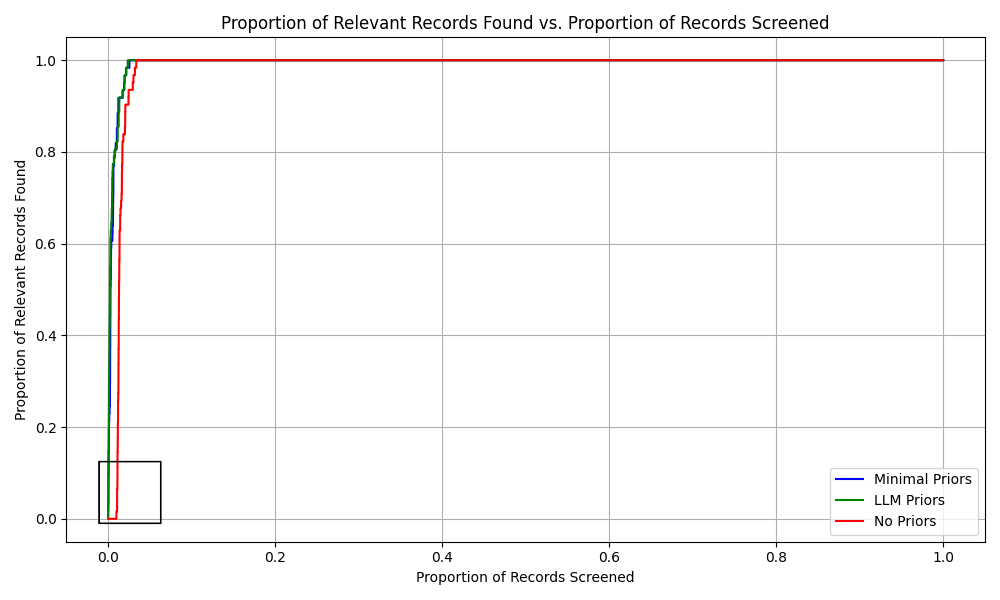
\includegraphics[width=0.9\textwidth]{../Report/images/zoomed_recall_plot.PNG}
  \caption{Recall plot of a single run of the true-example condition for the Brouwer (2019) dataset}
  \label{fig:zoomed-recall-plot}
\end{figure}


\clearpage

\subsection{Four recall plots of single runs of two datasets per condition (as didactic examples)}

Contain actual data but have been cherry-picked to show the differences between conditions. The goal is to show the reader what the recall plots look like and how they differ between conditions.

\begin{figure}[H]
     \centering
     \begin{subfigure}[b]{0.45\textwidth}
         \centering
         \includegraphics[width=0.9\linewidth]{../simulation_results/run_01/Brouwer_2019/recalls_plots/recall_plot_run_1_IVs_1_100_0.0.png}
         \caption{True examples condition (showing two quite differing recall curves)}
         \label{fig:TrueExamples}
     \end{subfigure}
     \hfill
     \begin{subfigure}[b]{0.45\textwidth}
         \centering
         \includegraphics[width=0.9\linewidth]{../simulation_results/run_01/Brouwer_2019/recalls_plots/recall_plot_run_2_IVs_1_100_0.4.png}
         \caption{Cold start condition (showing one entirely flat recall curve and one half flat recall curve)}
         \label{fig:ColdStart}
     \end{subfigure}
     \hfill
     \begin{subfigure}[b]{0.45\textwidth}
         \centering
         \includegraphics[width=0.9\linewidth]{../simulation_results/run_01/Brouwer_2019/recalls_plots/recall_plot_run_3_IVs_1_100_0.8.png}
         \caption{LLM condition (showing two decent recall curves, similar performance)}
         \label{fig:LLM}
     \end{subfigure}
     \hfill
     \begin{subfigure}[b]{0.45\textwidth}
         \centering
         \includegraphics[width=0.9\linewidth]{../simulation_results/run_01/Brouwer_2019/recalls_plots/recall_plot_run_4_IVs_1_500_0.0.png}
         \caption{Criteria-only condition (showing two decent recall curves, similar performance)}
         \label{fig:CriteriaOnly}
     \end{subfigure}
        \caption{Four recall plots of single runs of two datasets per condition (as didactic examples)}
        \label{fig:figures}
\end{figure}

\clearpage

\subsection{Aggregate recall plots with line for each condition, for two datasets}

The recall plots shown above are just examples of single runs. By simulating many many runs, we can obtain a more reliable estimate of the average performance of each condition. (i.e., do statistical analysis / significance testing).

\begin{figure}[htbp]
  \centering
  \includegraphics[width=0.45\textwidth]{aggregate_recall_plot_walker.png}
  \includegraphics[width=0.45\textwidth]{aggregate_recall_plot_moran.png}
  \caption{The number of relevant records found per dataset}
  \label{fig:walker-2018}
\end{figure}

\subsection{Boxplots of starting performance across all runs}

\begin{figure}[htbp]
  \centering
  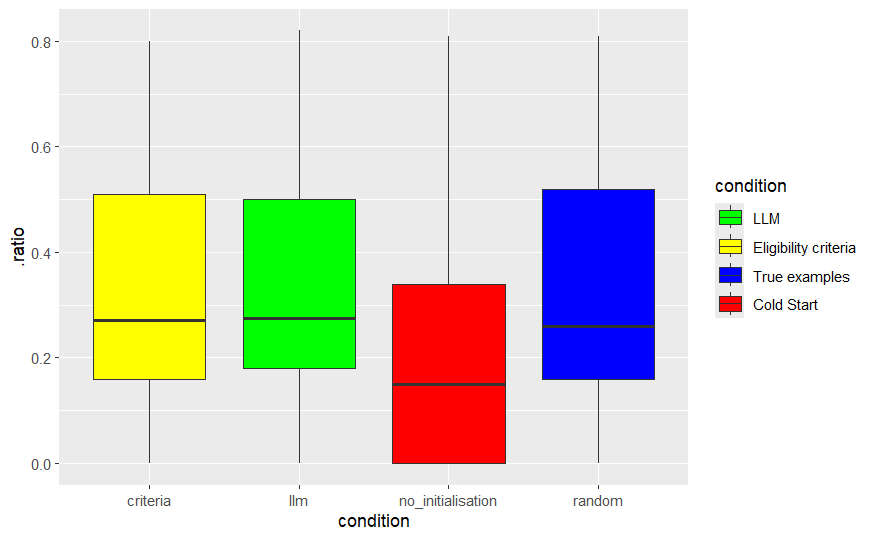
\includegraphics[width=0.45\textwidth]{../Report/images/example_boxplot.png}
  \caption{Example boxplot}
  \label{fig:boxplots-starting-performance}
\end{figure}

\subsection{Few sentences describing the results of the statistical analysis}

One alinea on reporting the statistical significance of the three contrasts: (1) LLM vs. cold-start, (2) criteria-only vs. cold-start, and (3) LLM vs. criteria-only.


\subsection{Additional analysis on using eligibility criteria as prior}

One alinea reporting the results of manually manipulating / enriching the elgibility criteria.

\section{Conclusion} 

The conclusion is that the cold start problem can be overcome by using the eligibility criteria of a systematic review to initialize the active learning model, and that LLM-generated examples do not improve starting performance beyond that achieved through initialisation using the systematic review's eligibility criteria criteria directly.


\section{Discussion}

\begin{enumerate}
  \item A limitating factor in the application of AI-assisted systematic reviews is the cold start problem. This is especially relevant to crisis situations such as COVID-19, where there may not be relevant prior literature and timely evidence synthesis is crucial.
  \item Prior research has shown that the cold start problem can be overcome by providing as little as one true pair example of a relevant paper and an irrelevant paper to the active learning model before screening begins \parencite{ferdinands2023performance,teijema2025large}. However, in some cases, there may be no prior examples of relevant papers available to initialize the model with. Moreover, the true examples a user has available may not be representative of the relevant papers in the systematic review, which may lead to suboptimal starting performance (i.e., bias / anchor effect -- ask Sixu).
  \item Currently, the cold start problem is typically addressed by consulting a domain expert to provide true examples of relevant papers to initialize the model with. However, this may not always be feasible, especially in crisis situations where timely evidence synthesis is crucial. (ask Ula -- EKE citations).
  \item Some limitations of the current study include:
    \begin{enumerate}
        \item Only a limited number of historical datasets were used. SYNERGY 2.0 coming soon!
        \item The of historical datasets. Future studies may consider addressing the cold start problem in a new systematic review.
        \item ...
    \end{enumerate}
  \item Practical implications of the current study include:
    \begin{enumerate}
        \item If no prior examples of relevant papers are available, the eligibility criteria of a systematic review can be used to initialize the active learning model and overcome the cold start problem. 
        \item Don't use LLMs. LLMs add very little at most and there are many disadvantages to their use.
        \item If one true example of a relevant paper is available, still use the eligibility criteria to initialize the model. This way your true paper can be used as a test for completeness of your screening (i.e., stopping rule is reached when the true example is found -- cite Tale \& Josien).
        \item ...
    \end{enumerate}
\end{enumerate}


% \begin{figure}[htbp]
%   \centering
%   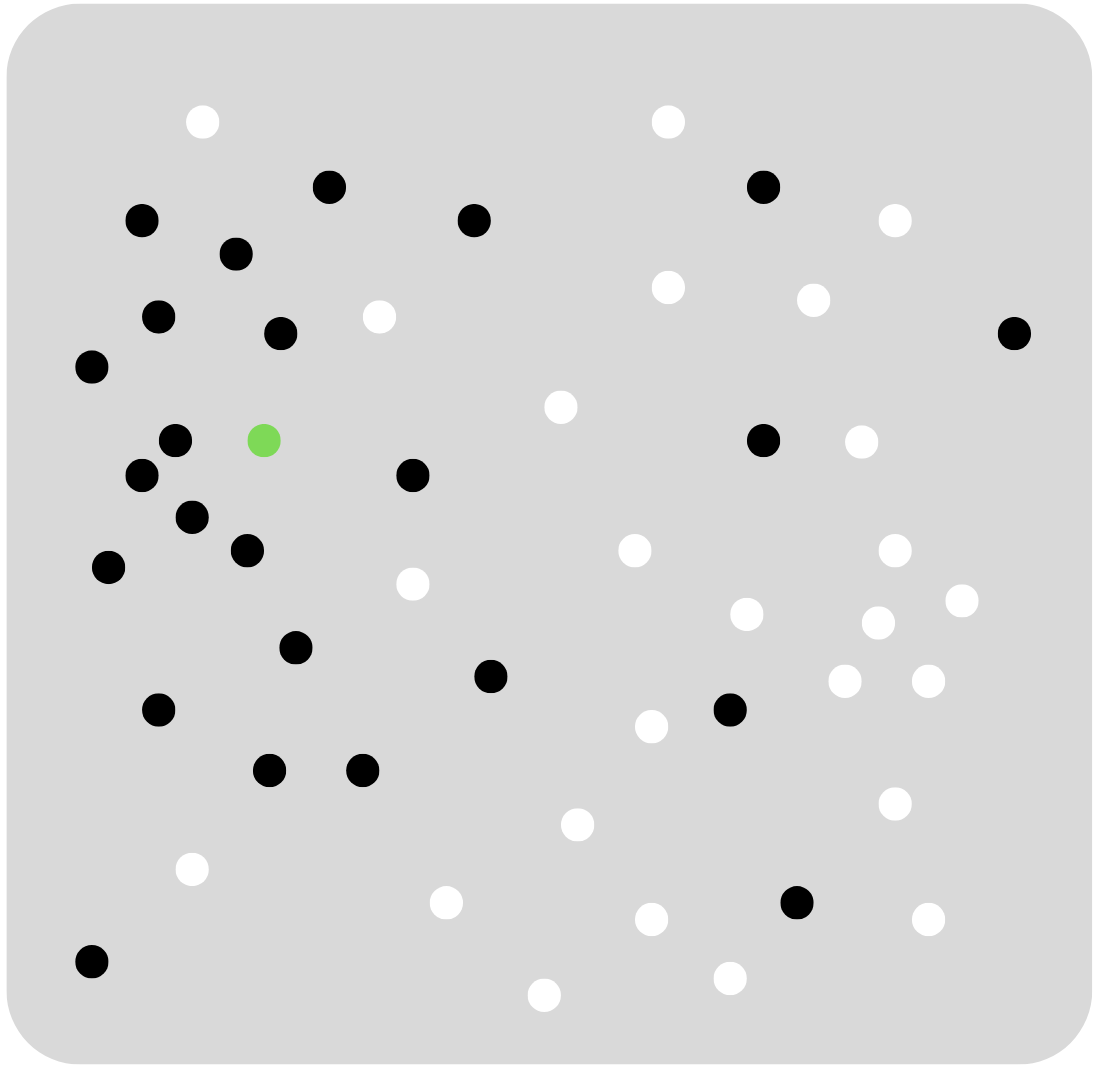
\includegraphics[width=0.2\textwidth]{vector_space/LLM_vector_space.png}
%   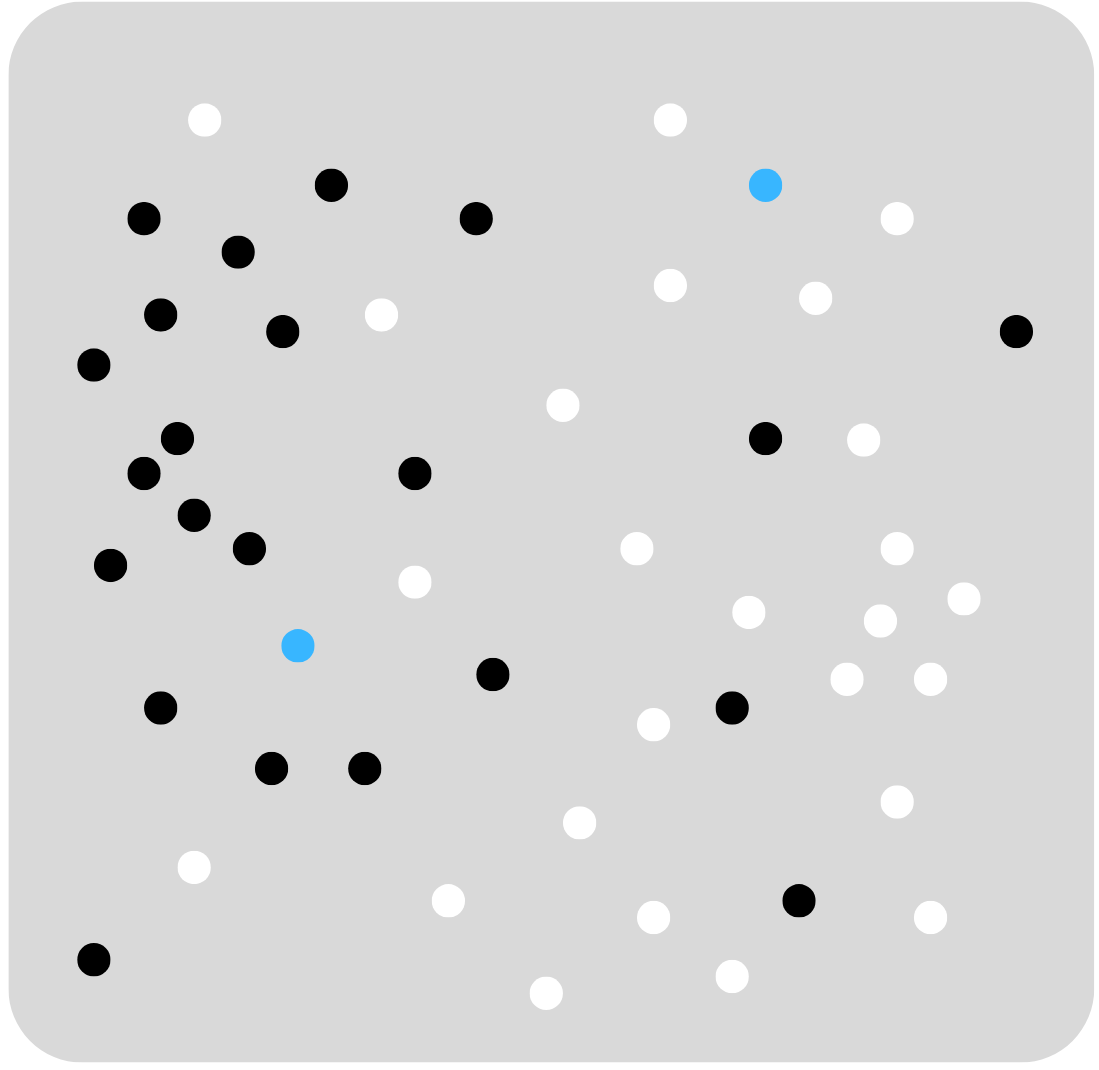
\includegraphics[width=0.2\textwidth]{vector_space/random_vector_space.png}
%   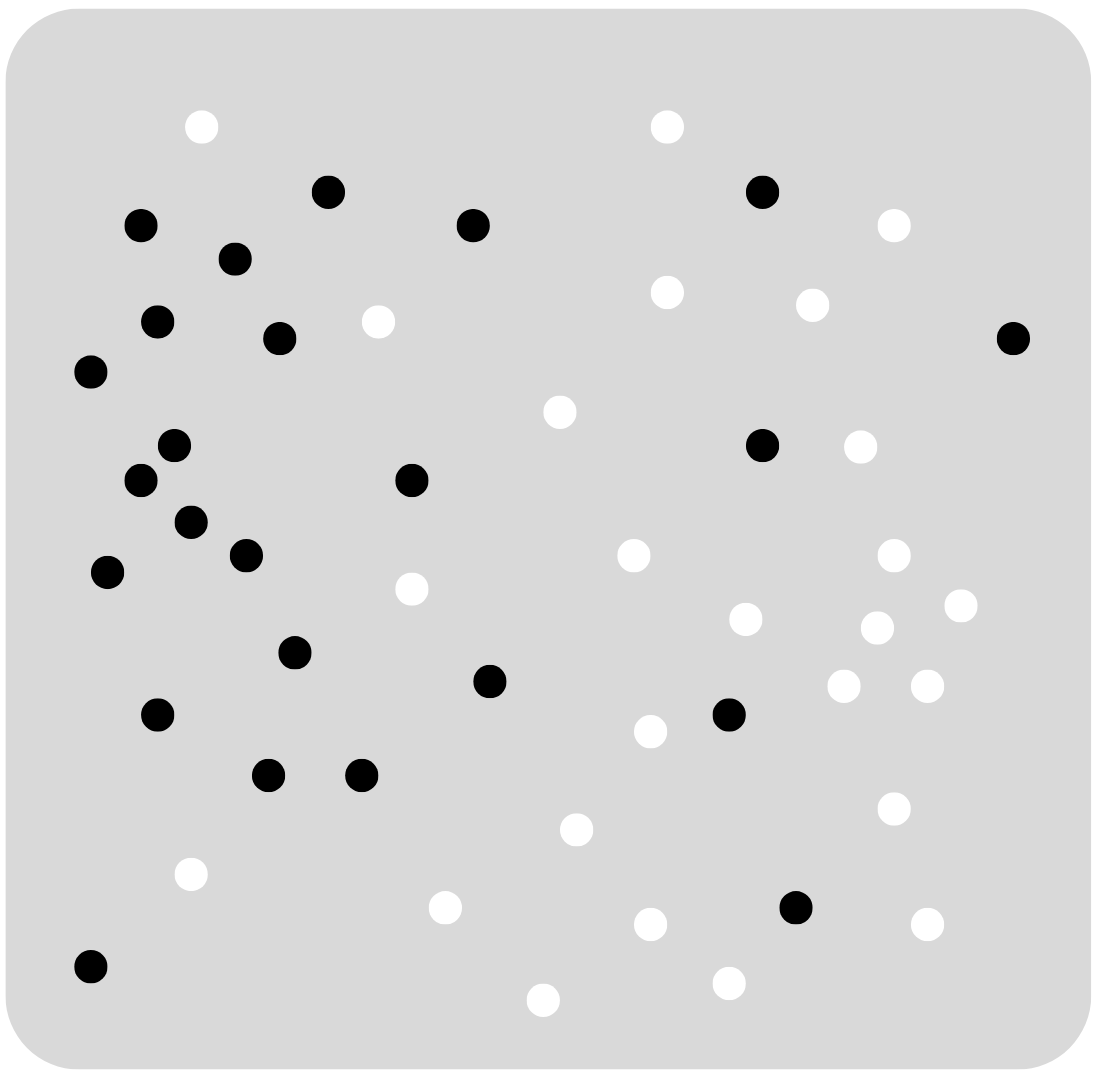
\includegraphics[width=0.2\textwidth]{vector_space/no_vector_space.png}
%   \caption{Ideal starting point for systematic reviews using active learning}
%   \label{fig:my-image}
% \end{figure}


% \subsubsection{Simulation design}

% In other words, whether, in the case of AI-assisted reviewing, prompt engineering actually aids in knowledge discovery or whether LLMs simply repackage existing knowledge.

% More LLM-specific variables were considered in advance (such as degree of jargon), however, because early simulations showed difference between the LLM- and criteria-based initialisation conditions, these variables were not further investigated. Future work may consider these variables in more detail.

% Most eligibility criteria are written in either conjunctive or disjunctive form. In the latter case, all the inclusion criteria must be met for a paper to be included, whereas in the former, only one must be met. This may affect how useful LLM-generated examples are compared to using the eligibility criteria directly or selecting random examples. This is because, for criteria in conjunctive form, abstracts will be relevant if and only if all the terms from the eligibility criteria are mentioned. In contrast, for criteria in in disjunctive form, the relevant abstracts will likely only contain one of the many terms mentioned in the eligibility criteria. 

% \subsubsection{Statistical Analysis}

% AI-assistant screening is actually sequence dependent. This is ignored by simply the summed successes and number of retrievals. Future work may consider modelling the sequence directly.

% The response variable makes sense to be viewed as a proportion and not a count because we know the true number of total relevant records. Future work modelling the retrieval of actual retrievals may more aptly consider it counts instead (e.g., Poisson).

% GLMM assume that the random effects are normally distributed (i.e., that the difference in starting performance between datasets follows a normal distribution). However, based on the results of a previous simulation study comparing the normalized loss performance of AI-assistant screening for different datasets, this seems unlikely \parencite{teijema2025large}. Future work may consider specifying a different random-effects distribution using hierarichal generalized linear models (HGLMs) or Bayesian methods.
% \subsection{Limitations}

% \begin{enumerate}
%     \item only one LLM used (gpt-4o-mini). Future work may consider other LLMs (e.g., open source LLMs).
%     \item Key limitation simulation study: data leakage (i.e., LLMs have been trained on synergy datasets). The ecological validity of the results are therefore somewhat limited.
%     \begin{enumerate}
%         \item There are two obvious solutions to the problem of data leakage: (1) apply the use of LLm-initialization on a new systematic review, and (2) use an older LLM from hugging face for example. 
%     \end{enumerate}
%     \item Another possible limitation: no switching of active leaning cycles (could fix contamination of synthetic data issue). 
%     \item The multilevel model assumption of heterogeneity between conditions may not hold. 
%     \item The effect of the length abstract may be small in part because this parameter had limited effect on the generated abstracts. However, since early analyses showed that the effect of the other LLM-specific parameters was limited (i.e., for temperature and number of abstracts), it is unlikely that the effect of length of abstract would be large either.
% \end{enumerate}

% Clusters should not be a problem because we only focus on starting performance (i.e., first 100 screened). Future work may consider the contamination hypothesis in more detail. 



\appendix

\section{SYNERGY metadata}

\begin{table}[ht]
\centering
\caption{Datasets overview}
\begin{tabularx}{\textwidth}{@{}r l X r r r@{}}
\toprule
\textbf{Nr} & \textbf{Dataset} & \textbf{Topic(s)} & \textbf{Records} & \textbf{Included} & \textbf{\%} \\
\midrule
1  & Appenzeller-Herzog\_2019 & Medicine & 2873  & 26  & 0.9 \\
2  & Bos\_2018                 & Medicine & 4878  & 10  & 0.2 \\
3  & Brouwer\_2019             & Psychology, Medicine & 38114 & 62  & 0.2 \\
4  & Chou\_2003                & Medicine & 1908  & 15  & 0.8 \\
5  & Donners\_2021             & Medicine & 258   & 15  & 5.8 \\
6  & Hall\_2012                & Computer science & 8793  & 104 & 1.2 \\
7  & Leenaars\_2019            & Psychology, Chemistry, Medicine & 5812  & 17  & 0.3 \\
8  & Leenaars\_2020            & Medicine & 7216  & 583 & 8.1 \\
9  & Meijboom\_2021            & Medicine & 882   & 37  & 4.2 \\
10 & Menon\_2022               & Medicine & 975   & 74  & 7.6 \\
11 & Moran\_2021               & Biology, Medicine & 5214  & 111 & 2.1 \\
12 & Muthu\_2021               & Medicine & 2719  & 336 & 12.4 \\
13 & Nelson\_2002              & Medicine & 366   & 80  & 21.9 \\
14 & Oud\_2018                 & Psychology, Medicine & 952   & 20  & 2.1 \\
15 & Radjenovic\_2013          & Computer science & 5935  & 48  & 0.8 \\
16 & Sep\_2021                 & Psychology & 271   & 40  & 14.8 \\
17 & Smid\_2020                & Computer science, Mathematics & 2627  & 27  & 1.0 \\
18 & van\_de\_Schoot\_2018     & Psychology, Medicine & 4544  & 38  & 0.8 \\
19 & van\_der\_Valk\_2021      & Medicine, Psychology & 725   & 89  & 12.3 \\
20 & van\_der\_Waal\_2022      & Medicine & 1970  & 33  & 1.7 \\
21 & van\_Dis\_2020            & Psychology, Medicine & 9128  & 72  & 0.8 \\
22 & Walker\_2018              & Biology, Medicine & 48375 & 762 & 1.6 \\
23 & Wassenaar\_2017           & Medicine, Biology, Chemistry & 7668  & 111 & 1.4 \\
24 & Wolters\_2018             & Medicine & 4280  & 19  & 0.4 \\
\bottomrule
\end{tabularx}
\caption{Please note that two of the datasets included in the original SYNERGY dataset were excluded entirely due to data quality issues: Chou (2003) and Jeyaraman (2020). For one dataset (Moran, 2021), an updated version was used due to data quality issues in the original version.}
\end{table}
\label{tab:SYNERGY}

% \section{Format exported simulation results} \label{sec:format_exported_simulation_results}

% Each simulation run is stored in a separate CSV file. Every row represents a screened paper and contains the following information:

% \begin{enumerate}[label=\arabic*), leftmargin=*, nosep]
%   \item The paper's record ID,
%   \item The assigned label (i.e., relevant or irrelevant),
%   \item The classifier, querier, balancer and feature extractor used,
%   \item The size of the training set,
%   \item A time tag.
% \end{enumerate} 

% Furthermore, the following naming convention is used for the CSV files: \newline condition\_run\_run\_IVs\_n\_abstracts\_length\_abstracts\_llm\_temperature.csv. The same naming convention is used for the recall plots of each simulation run and for the generated abstracts in the LLM initialisation condition.

% Finally, at the end of each run, the current values of the input parameters, the outcome variables and other relevant metadata are appended to a long format master dataframe for analysis. The columns of this dataframe are as follows:

% \begin{enumerate}[label=\arabic*), leftmargin=*, nosep]
%     \item the name of the outcome variable
%     \item the value of the outcome variable
%     \item name of the simulated dataset,
%     \item the condition,
%     \item the values of the independent variables (NaN for the control conditions):
%         \begin{enumerate}
%         \item number of abstracts
%         \item length of the abstracts
%         \item temperature settings of the llm (i.e., diversity)
%         \end{enumerate}
%     \item timestamp
%     \item the run number
% \end{enumerate}

% This yields a data-frame containing one observation for each combination of dataset (n=26), condition (n=3), independent variables and their levels (n=$3 \times 4 \times 4 \times 5 \times 5 = 1200$), and run (n=1), thus with $26 \times 3 \times 1200 \times 1 = 93600$ rows, and the 12 columns enumerated above. 

% \section{Padding} \label{sec:padding}

% It is worth noting that the simulation may stop prematurely if all the relevant records are found before the stopping rule is reached (e.g. after screening 100 records). To accurately emulate a researcher who is unaware that all the relevant records have been found and therefore continues screening until the stopping rule is reached, the simulation results were supplemented with rows containing the label 'zero' (i.e. irrelevant records) until the stopping rule would have been reached. This process is referred to as 'padding' and ensures that the final simulation results are accurate.


% References
\printbibliography
%TC:endignore

\end{document}
